\section{Methods}
	\begin{multicols*}{2}
		[\subsection{\gls{SRS} analysis}
		\gls{SDLC} starts with eliciting the \gls{SRS}, noted by the stakeholders. As stakeholders use their own language to state their requirements, it is observed to be very often ambiguous and confusing to analyze and subsequently design the desired solution. On one side we only focus on \gls{SRS} requirement document which follows the IEEE-STD-830 standard in a textual form. In the other side \gls{NLP} concepts are found to be helpful for the analysis. \gls{NLP} system processes the data written in natural language in an intelligent manner and generates an information which is comparatively easier to analyze.\cite{Tripathy}]
		Using \gls{NLP} can help in:
		\begin{itemize}
			\item the syntax of natural language
			\item the lexical context of the words
			\item the semantic components which construct the literal meaning of a sentence
			\item the pragmatic components which construct non-literal meaning of a sentence
			\item the parser generating the phrase tree structure of a sentence.
		\end{itemize}
		\gls{POST} is a semantic analysis approach and deals with assigning one or more \gls{POS} to a given word. The different types of \gls{POS} are,
		\begin{itemize}
			\item Noun (names): a word or lexical item denoting any abstract (abstract noun: e.g. home) or concrete entity (concrete noun: e.g. house); a person (police officer, Michael), place (coastline, London), thing (necktie, television), idea (happiness), or quality (bravery). Nouns can also be classified as count nouns or non-count nouns; some can belong to either category. The most common part of speech; they are called naming words.
			\item Pronoun (replace or again placed): a substitute for a noun or noun phrase (them, he). Pronouns make sentences shorter and clearer since they replace nouns.
			\item Adjective (describes, limits): a modifier of a noun or pronoun (big, brave). Adjectives make the meaning of another word (noun) more precise.
			\item Verb (states action or being): a word denoting an action (walk), occurrence (happen), or state of being (be). Without a verb a group of words cannot be a clause or sentence.
			\item Adverb (describes, limits): a modifier of an adjective, verb, or another adverb (very, quite). Adverbs make language more precise.
			\item Preposition (relates): a word that relates words to each other in a phrase or sentence and aids in syntactic context (in, of). Prepositions show the relationship between a noun or a pronoun with another word in the sentence.
			\item Conjunction (connects): a syntactic connector; links words, phrases, or clauses (and, but). Conjunctions connect words or group of words.
			\item Interjection (expresses feelings and emotions): an emotional greeting or exclamation (Huzzah, Alas). Interjections express strong feelings and emotions.
			\item Article (describes, limits): a grammatical marker of definiteness (the) or indefiniteness (a, an). The article is not always listed among the parts of speech. It is considered by some grammarians to be a type of adjective or sometimes the term 'determiner' (a broader class) is used.
		\end{itemize}
		Identification of all these \gls{POS} makes the task of \gls{NLP} simpler.
		
		Following Fillmore’s idea of defining a universal set of cases and Nan Niu’s variation structure, we introduce a set of extended dimensions for conceptualizing the functional variability structure. An \gls{EFRF} is composed by 10 different semantic cases. Thus, we consider the following variation dimensions for an \gls{EFRF}.
		\begin{itemize}
			\item Agentive defines the agent whose activities will occur in \gls{EFRF}’s affairs. For example, $\{\mbox{student}\}_{Agentive}$
			“do homework”.
			\item Action defines the main action of the activity. For
			example, “TA” $\{\mbox{mark}\}_{Action}$.
			\item Objective defines the object affected by the activity.
			For example, “mark” $\{\mbox{homework}\}_{Objective}$.
			\item Agentmod defines the feature of agent. For example,
			{Senior}Agentmod $\{\mbox{student}\}_{Agentive}$.
			\item Objmod defines the feature of object. For example,
			$\{\mbox{c++}\}_{Objmod} \{\mbox{homework}\}_{Objective}$.
			 \item Locational defines the location where the \gls{EFRF} affairs occur. For example, “do homework” $\{\mbox{at home}\}_{Locational}$.
			 \item Temporal defines the duration or frequency of the
			 \gls{EFRF}’s activity. For example, “mark homework” $\{\mbox{every Sunday}\}_{Temporal}$.
			 \item  Manner defines the way or tool by which the
			 \gls{EFRF}’s activity is performed. Some examples are,
			 “access Internet” via $\{\mbox{Ethernet, Wireless}\}_{Manner}$,
			 “mark assignment” through $\{\mbox{Internet}\}_{Manner}$.
			 \item Goal defines the goal of the \gls{EFRF}’s activity. For example, “do homework carefully” $\{\mbox{in order to get an A}\}_{Goal}$.
			 \item Constraint defines the requirement and constraint
			 that make the activity occur. For example, “do
			 homework on-line” if $\{\mbox{access Internet}\}_{Constraint}$.
		\end{itemize}
		This extended set reflects most grammatical features
		that are associated with functional requirements description;
		hence it can serve as a framework of categories that helps
		analysts understand the variation points, i.e. what can vary,
		of the \gls{EFRF}. The systematical and clear definition of these
		variable points can help the effectiveness of software product line's functional variability modeling. 
		
		\begin{minipage}{\linewidth}
			\centering
			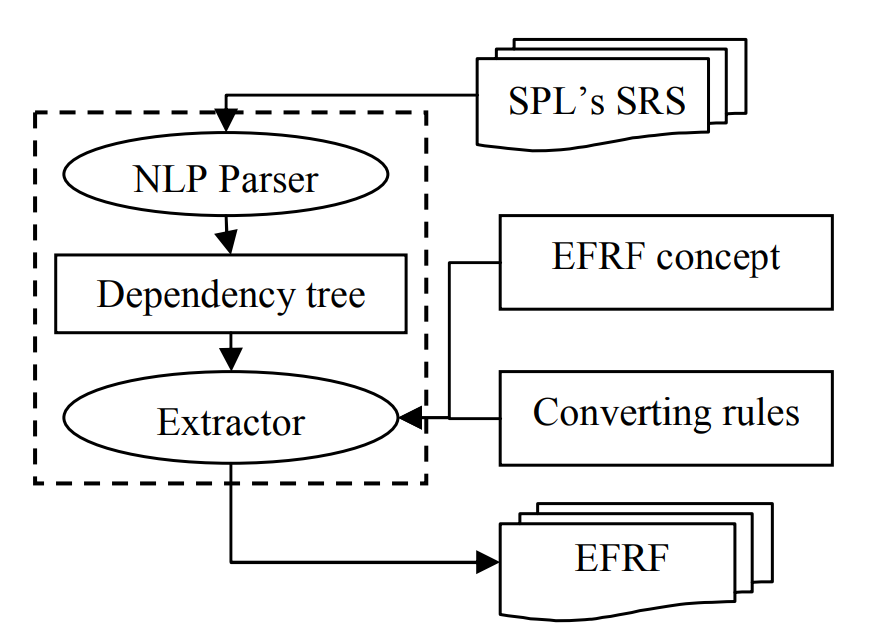
\includegraphics[width=\linewidth]{Architecture.png}
			\caption{Architecture}
			\label{fig:cc}
		\end{minipage}
		
	\end{multicols*}


\begin{minipage}{\linewidth}
	\begin{multicols*}{2}
		[
		\vspace{6 mm}
		\subsection{Semantic Analyzer}
		Despite provides construct that to machine instructions, it provides enough abstraction above \gls{asm} for developers to finish their work independently of platform  on which their C program runs.		C provides just enough abstraction above assembly language for
		programmers to get their work done without having to worry about
		the details of the machines on which the programs run. Despite
		this abstraction, C is also known for the ease in which it allows
		programmers to write buggy programs. With no runtime checks
		and little static checking, in C the programmer is to be trusted
		entirely. Despite the abstraction, the language is still low-level
		enough that programmers can take advantage of assumptions about
		the underlying architecture. Trust in the programmer and the ability
		to write non-portable code are actually two of the design principles
		under which the C standard was written. These ideas often work
		in concert to yield intricate, platform-dependent bugs. The potential
		subtlety of C bugs makes it an excellent candidate for formalization,
		as subtle bugs can often be caught only by more rigorous means.]
		In this paper, we present a formal semantics of MISRA-C that can be used
		for finding bugs, since it has just enough restriction to present fully proved formal semantic. 
	\end{multicols*}
\end{minipage}

\begin{minipage}{\linewidth}
	\begin{multicols*}{2}
		[
		\vspace{6 mm}
		\subsection{Consistency Check}
		Temp]
		Temp.
	\end{multicols*}
\end{minipage}

